\documentclass[tikz,border=5pt]{standalone}
\usepackage{tikz}
\usepackage{amsmath}
\usetikzlibrary{arrows.meta,calc,positioning}
\definecolor{nebula}{HTML}{6366F1}
\definecolor{spark}{HTML}{14B8A6}
\definecolor{ink}{HTML}{334155}
\begin{document}
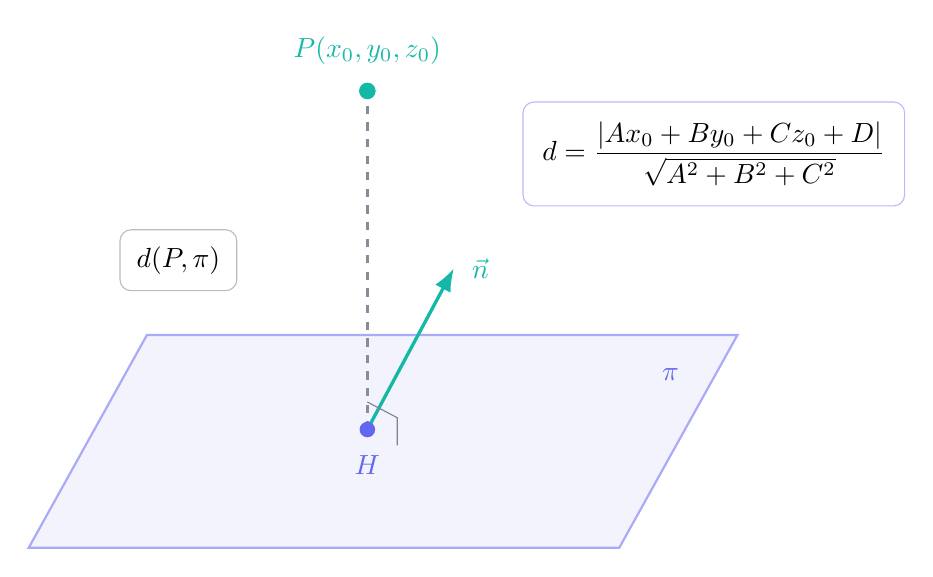
\begin{tikzpicture}[font=\sffamily,>=Latex]
  \fill[nebula!8] (-4,-1.5)--(3.5,-1.5)--(5,1.2)--(-2.5,1.2)--cycle;
  \draw[nebula!55,thick] (-4,-1.5)--(3.5,-1.5)--(5,1.2)--(-2.5,1.2)--cycle;
  \node[nebula] at (4.15,.7) {$\pi$};
  \coordinate (H) at (.3,0);
  \coordinate (P) at (.3,4.3);
  \draw[dashed,very thick,ink!60] (H)--(P);
  \draw[->,very thick,spark] (H)--++(1.1,2.05) node[right=5pt,fill=white,inner sep=1pt] {$\vec n$};
  \fill[nebula] (H) circle (2.8pt) node[below=6pt] {$H$};
  \fill[spark] (P) circle (3pt) node[above=6pt] {$P(x_0,y_0,z_0)$};
  \draw[ink!65] (.3,.35)--(.68,.15)--(.68,-.2);
  \node[draw=ink!35,rounded corners=4pt,fill=white,inner sep=6pt] at (-2.1,2.15) {$d(P,\pi)$};
  \node[draw=nebula!45,rounded corners=4pt,fill=white,inner sep=7pt] at (4.7,3.5)
    {$\displaystyle d=\frac{|Ax_0+By_0+Cz_0+D|}{\sqrt{A^2+B^2+C^2}}$};
\end{tikzpicture}
\end{document}
